\begin{example}{alternate way to simulate the bouncing ball}
\label{ex:bbblocks}

Consider the bouncing ball system with a constant input and regular data as given in Example~\IfSAE{1.3}{\ref{ex:bbinput}}. This example shows that a MATLAB function block, such as the jump set {\em D}, can be replaced with operational blocks in Simulink. Figure~\ref{fig:bbblocks} shows this implementation. The other functions and solutions are the same as in Example~\IfSAE{1.3}{\ref{ex:bbinput}}.

\begin{figure}[ht]
  \begin{center}
    {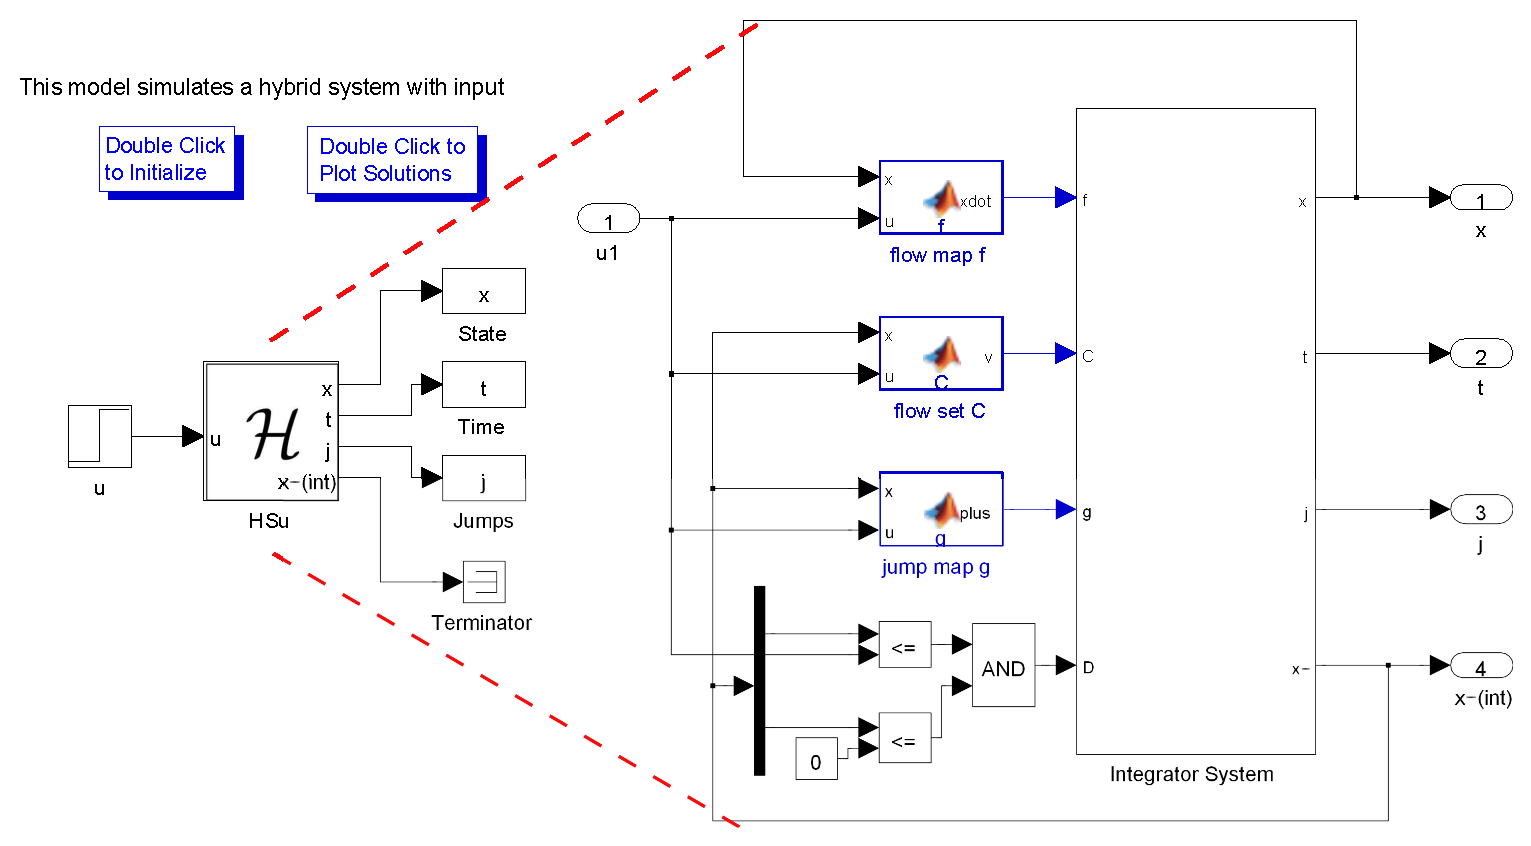
\includegraphics[width=.95\textwidth]{figures/Simulink/HybridSimulatorBBblocks}}
   \caption{Simulink implementation of bouncing ball example with operator blocks}
\label{fig:bbblocks}
  \end{center}
\end{figure}

For MATLAB/Simulink files of this example, see Examples/Example\_1.3 and Examples/Example\_1.4.

\end{example}
